\section{Methods}

\subsection{Data Operationalization}

To evaluate the diachronic dynamics of paradigm leveling, we constructed a dataset amalgamating attestations from the Middle High German and Early New High German corpora. The data tracks the binary outcome of whether a specific vowel or consonant alternation has been leveled compared to its historical baseline and modern reflexes. The primary variables are operationalized as follows:

\textbf{- Outcome} (\textsc{has\_levelled}): A binary variable where $1$ indicates the historically expected alternation has been replaced (leveled), and $0$ indicates it is preserved.

\textbf{- Time} (\textsc{date}): The approximate year of the document's composition.

\textbf{- Lemma ID} (\textsc{lemma\_std}): A unique identifier linking derived forms of a verb across both corpora.

\textbf{- Document ID} (\textsc{id}): A proxy for scribal identity to account for individual textual idiosyncrasies.

\textbf{- Marking Type} (\textsc{marking\_type}): A three-level categorical variable combining the specific morphological element under observation and the structural bipartiteness of the paradigm (\textit{vowel\_unipartite}, \textit{vowel\_bipartite}, \textit{consonant\_bipartite}).

\textbf{- Lemma Frequency} (\textsc{log\_freq}): The log-transformed lemma frequency of the verb. Computed by observing all the forms corresponding to a lemma and summing their individual frequencies. We also fit a model with token frequency. Please note that token frequency is defined as the average form frequency across the forms from past singular subparadigm and the forms from past plural subparadigm.\footnote{Due to data sparsity we are worried that using individual forms' frequencies would be too noisy in terms of the signal.} 

\textbf{- Alternation Presence} (\textsc{has\_alt\_pres}, \textsc{has\_alt\_past}): Binary dummy variables indicating the presence of an alternation between the present and past singular subparadigm, or the past singular and past plural subparadigm, respectively.

\textbf{- Alternation Type Frequency} (\textsc{log\_alt\_pres\_freq}, \textsc{log\_alt\_past\_freq}): The log-transformed type frequency of the specific alternation pattern (e.g., the exact vocalic \textit{a $\sim$ e} or consonantal \textit{d $\sim$ t} pattern) within a given regional variety.

\textbf{- Inflectional Context} (\textsc{std\_infl}): The morphological cell observed. As described above, High German paradigms in our dataset are binned into two categories: (1) indicative past singular subparadigm that includes 1st and 3rd person forms and (2) indicative past plural subparadigm that includes all plural variants and the second person singular past indicative.

\textbf{- Variety} (\textsc{variety}): The macro-regional dialect class (Central German or Upper German).

\begin{table}[ht]
\centering
\renewcommand{\arraystretch}{1.4} % Matches the vertical padding of the original table
\setlength{\tabcolsep}{24pt}      % Adjusts cell width to look spacious
\begin{tabular}{|l|l|}
\hline
\multicolumn{2}{|c|}{\textbf{Past indicative}} \\ \hline
ich verl\={o}s & \cellcolor{tablegrey}wir verlurn \\ \hline
\cellcolor{tablegrey}du verl\"{u}r & \cellcolor{tablegrey}ir verlurt \\ \hline
\"{e}r verl\={o}s & \cellcolor{tablegrey}sie verlurn \\ \hline
\end{tabular}
\caption{Middle High German paradigm of \textit{verlieren}. The shaded cells indicate what is called "past plural subparadigm" throughout the paper, and the non-shaded cells refer to "past singular subparadigm".}
\end{table}

\subsection{Modeling Architecture and Theoretical Assumptions}

Any statistical model attempting to capture the breakdown of the \textit{Grammatischer Wechsel} must mathematically operationalize the cognitive and systemic pressures defined by Paul's Principle. The foundational assumption underlying this modeling endeavor is that analogical change is a probabilistically constrained process governed by observable variables. The primary theoretical assumption is that bipartite marking creates a threshold of resistance against leveling, decreasing its overall probability.

To adequately capture this breakdown, our model must evaluate differences between vowels and consonants alongside the structural layout of the paradigm. However, note that the element (consonant or vowel) that is evaluated for being levelled or not, is highly predictive of its bipartiteness. By definition, the consonants in non-bipartite verbs are not subject to levelling and hence not included in the dataset. This creates the multicollinearity problem between these two variables. To resolve this structural dependency, we combine them into a single joint variable, \textsc{marking\_type}. This allows us to directly estimate the distinct diachronic trajectories of unipartite vowels, bipartite vowels, and bipartite consonants without estimating impossible interaction states. In a more conceptual sense, we can only observe the effect of bipartite marking on vowels, as that's the only element which shows up in bipartite and non-bipartite verbs, as opposed to consonants. 

Furthermore, we introduce stringent controls for alternation type frequency. It is plausible that the survival of a specific allomorphic alternation is driven not strictly by its bipartite structure, but simply by how broadly distributed that specific phonological pattern (e.g., an \textit{a $\sim$ e} vowel gradation or an \textit{s $\sim$ r} consonant alternation) is across the verbal lexicon. By including both a dummy variable for the presence of an alternation and a continuous log-transformed measure of its type frequency across lemmas, we can isolate the true effect of Paul's Principle and discard type frequency as an exclusive alternative explanation for the observed behavior. It should be noted that the two alternation presence dummies are very unevenly distributed. Only 40 of the 13,184 modeling observations lack an alternation between the present and past singular subparadigms, so \textsc{has\_alt\_pres} carries little information and its coefficient is largely determined by the prior. The corresponding contrast for \textsc{has\_alt\_past} is well populated, with 2,553 observations against 10,631.

Lemma frequency often acts as a conserving force and is therefore included. Critically, we expect the protective effects of frequency to dynamically shift over historical time. To rigorously capture this temporal interaction, we utilize a tensor product smooth. While simple temporally conditioned smooths can capture parallel curves, a tensor product explicitly models the complex, two-dimensional interaction surface between time and frequency. Extensive model comparison utilizing Leave-One-Out Cross-Validation (LOOCV) \citep{vehtari2017practical} confirmed that the tensor product formulation significantly outperforms simpler smooths, making it the primary model reported in this analysis.

For geographical variation, documents were assigned to Central German or Upper German macrovariety. We decided to go with macrovarieties as opposed to more granular dialectal taxonomy as there is a significant sparsity in the data. Moreover, the two corpora that were used do not have a single unified dialect division either, so this would require deeper philological inspection of individual documents to accurately attribute it to a particular dialect. Due to different socio-historical circumstances, we expect the temporal dynamics to diverge for the two macrovarieties. Finally, the model accounts for the idiosyncratic properties of individual lemmas and scribes via random intercepts. 

\subsection{Mathematical Specification of the Bayesian Model}

To map the theoretical constraints onto a rigorous statistical framework, we utilize a Bayesian Generalized Additive Mixed Model (GAMM) with a Bernoulli likelihood and logit link function. Let $y_i \in \{0, 1\}$ represent the leveling status for observation $i$. The probability of leveling, $p_i$, is modeled as:
$$y_i \sim \text{Bernoulli}(p_i)$$
$$\text{logit}(p_i) = \eta_i$$
The linear predictor $\eta_i$ structurally partitions the variance into baseline fixed effects, non-linear dynamic smooths over time, complex tensor products, and group-level random effects:
$$\eta_i = \beta_0 + \beta_1 \text{Marking}_i + \beta_2 \text{Freq}_i + \beta_3 \text{HasPres}_i + \beta_4 \text{LogPresFreq}_i + \beta_5 \text{HasPast}_i + \beta_6 \text{LogPastFreq}_i$$ 
$$+ \beta_7 \text{Infl}_i + \beta_8 (\text{Infl}_i \times \text{Mark}_i)$$
$$+ s_1(\text{date}_i) + s_2(\text{date}_i, \text{by} = \text{Mark}_i) + t_2(\text{date}_i, \text{Freq}_i) + s_3(\text{date}_i, \text{by} = \text{Infl}_i) + s_4(\text{date}_i, \text{by} = \text{Var}_i)$$
$$+ \alpha_{\text{Var}[i]} + \alpha_{\text{Lemma}[i]} + \alpha_{\text{ID}[i]}$$

Where:
\begin{itemize}
    \item \textbf{$\text{Marking}_i$} is the three-level categorical indicator of marking type (\textit{vowel\_unipartite}, \textit{vowel\_bipartite}, \textit{consonant\_bipartite}).
    \item \textbf{$\text{Freq}_i$} denotes log-transformed lemma or token frequency.
    \item \textbf{$\text{HasPres}_i$} and \textbf{$\text{HasPast}_i$} are binary indicators for the presence of alternations in present/past singular subparadigms or between past singular/past plural subparadigms, respectively.
    \item \textbf{$\text{LogPresFreq}_i$} and \textbf{$\text{LogPastFreq}_i$} are the log-transformed type frequencies of those respective alternations.
    \item \textbf{$\text{Infl}_i$} represents the inflectional subparadigm in the respective row.
    \item \textbf{$\text{Var}_i$} represents the geographical variety.
    \item \textbf{$s(\cdot)$} functions represent thin-plate regression splines capturing non-linear diachronic trajectories. The argument \textit{by} allows the temporal dynamics to vary depending on the levels of a categorical variable. For the final model, we utilize $k=10$ basis functions to provide sufficient flexibility for the splines to capture complex historical curves without aggressively overfitting. Note that we have also fitted a model with $k=4$, the results for which are reported in the appendix. The models are largely the same in their results but the model with higher $k$ value is preferred via model comparison.
    \item \textbf{$t_2(\cdot)$} represents a tensor product smooth, allowing for a fully interactive, two-dimensional surface between the document date and the lemma's frequency.
    \item \textbf{$\alpha$} terms capture random intercepts for macro-variety, specific lemmas, and individual scribal documents.
\end{itemize}

The parameters are regularized utilizing weakly informative priors, stabilizing the posterior geometry and preventing extreme estimates characteristic of complete separation:
$$\beta_0 \sim \text{Normal}(0, 1.5)$$
$$\beta_k \sim \text{Normal}(0, 1) \quad \text{for } k \in \{1, 2, \dots, 8\}$$
$$\sigma_{\alpha} \sim \text{Exponential}(2)$$
$$\sigma_{s} \sim \text{Exponential}(2)$$
The exponential priors on the standard deviations ($\sigma$) act as a regularizing penalty against excessively large group-level variations or overly ``wiggly'' spline trajectories, assuming most effects cluster reasonably close to the average unless strongly supported by the data. This formal specification isolates the diachronic pressures predicted by Paul's Principle while safely marginalizing extraneous socio-historical noise and item-level idiosyncrasies.

We fitted all the models using Stan \citep{Carpenteretal2017} via the {\tt brms} interface \citep{brms} in R. Stan implements the No U-Turn Sampler (NUTS) version of the Markov Chain Monte-Carlo algorithm. The models ran for four chains of 4000 iterations each, out of which 2000 iterations per chain were discarded as warm-up for the MCMC. We set the {\tt adapt\underline{\phantom{x}}delta} argument to $0.99$, which decreases the step size of the sampler and mitigates divergence across chains, and allowed for a maximum tree depth of $10$. All five models converged, with a maximum $\hat{R}$ of $1.009$ and $\hat{R} \le 1.01$ across 100\% of estimated parameters. The lowest bulk and tail effective sample sizes across models were $777$ and $634$ respectively, and divergent transitions ranged from $0$ to $9$ per model out of $8000$ post-warmup draws. Model comparison was executed using Pareto-smoothed importance sampling Leave-One-Out Cross-Validation (PSIS-LOO).


\pagebreak

\section{Results}

To empirically test Paul's Principle and the dynamics of paradigm leveling, we evaluated five Bayesian Generalized Additive Mixed Models (GAMMs) with varying degrees of complexity. The models evaluated the binary outcome of whether a historically expected alternation was leveled or preserved. 

\subsection{Model Comparison and Evaluation}
Model comparison was conducted using Leave-One-Out Cross-Validation (LOO-CV).

The tensor product model, which specified a fully interactive tensor product between the document date and the lemma's frequency demonstrated the best fit to the data. The model with $k=4$ basis functions and smooth interaction performed the worst (\texttt{elpd\_diff} = -51.2, LOOIC = 2320.3). The superior performance of the tensor model confirms that the diachronic pressures of frequency on analogical change are not strictly parallel over time, but interact dynamically across the centuries. Consequently, the results reported below are primarily derived from the top-performing tensor model with lemma frequency. The results from other models are shown in the appendix. All in all, the effects are largely the same across all models and the directionality of the effect and/or their credible intervals' overlap with zero is also the same across models.

\begin{table}[h]
\centering
\caption{Model Comparison Results}
\label{tab:model_comparison}
\begin{tabular}{lcccccc}
\toprule
 & \textbf{elpd\_diff} & \textbf{se\_diff} & \textbf{elpd\_loo} & \textbf{se\_elpd\_loo} & \textbf{looic} & \textbf{se\_looic} \\
\midrule
\textbf{Tensor (k=10)} & 0.0 & 0.0 & -1108.9 & 48.6 & 2217.9 & 97.2 \\
\textbf{Smooth interaction (k=10)}    & -15.7 & 5.2 & -1124.6 & 49.1 & 2249.3 & 98.3 \\
\textbf{Tensor | Token Freq. (k=10)}    & -20.1 & 6.1 & -1129.0 & 49.0 & 2258.0 & 97.9 \\
\textbf{Tensor (k=4)} & -49.3 & 8.3 & -1158.2 & 49.5 & 2316.5 & 99.0 \\
\textbf{Smooth interaction (k=4)}   & -51.2 & 9.3 & -1160.1 & 49.8 & 2320.3 & 99.7 \\
\bottomrule
\end{tabular}
\end{table}

\subsection{Temporal Dynamics of Paradigm Leveling}
The temporal trajectory of paradigm leveling in High German strong verbs exhibits a classic S-curve of language change shown in Figure \ref{fig:date_effect}. The conditional effects over time indicate that the system remained highly stable, with leveling probabilities sitting near zero until approximately 1300 CE. Following 1300 CE, the probability of morphological homogenization accelerated sharply, peaking toward the end of the Early New High German (ENHG) period (circa 1500 CE). 

\begin{figure}
    \centering
    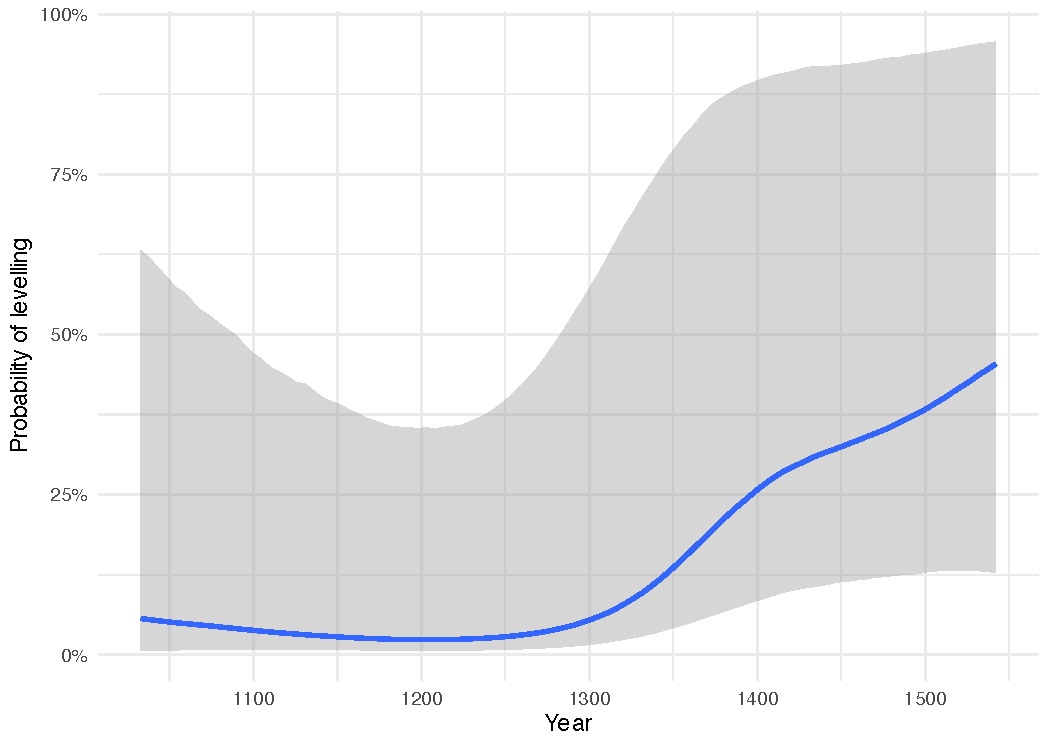
\includegraphics[width=0.75\linewidth]{figures/date_effect.pdf}
    \caption{The probability of levelling over time.}
    \label{fig:date_effect}
\end{figure}

\subsection{Evaluating Paul's Principle: The Role of Bipartite Marking}
The central hypothesis of this study -- Paul's Principle -- predicts that verbs with redundant, bipartite marking will establish a higher cognitive threshold of resistance against leveling compared to unipartite paradigms. Our findings provide no support for this Neogrammarian observation. To check whether there is any difference between the levelling log-odds of vowels in unipartite verbs and of vowels in bipartite verbs, we calculate the difference in their effects on the probability of levelling using evidence ratios\footnote{Using function {\sc hypothesis}: https://paulbuerkner.com/brms/reference/hypothesis.brmsfit.html} as implemented in {\sc brms}. The evidence ratio for a difference is only 0.44; the CI difference in effects is $[-2.04, ~1.02]$. The lack of the effect across both dialectal macro-regions is also illustrated in Figure \ref{fig:bi_uni_diff}. 

\begin{figure}
    \centering
    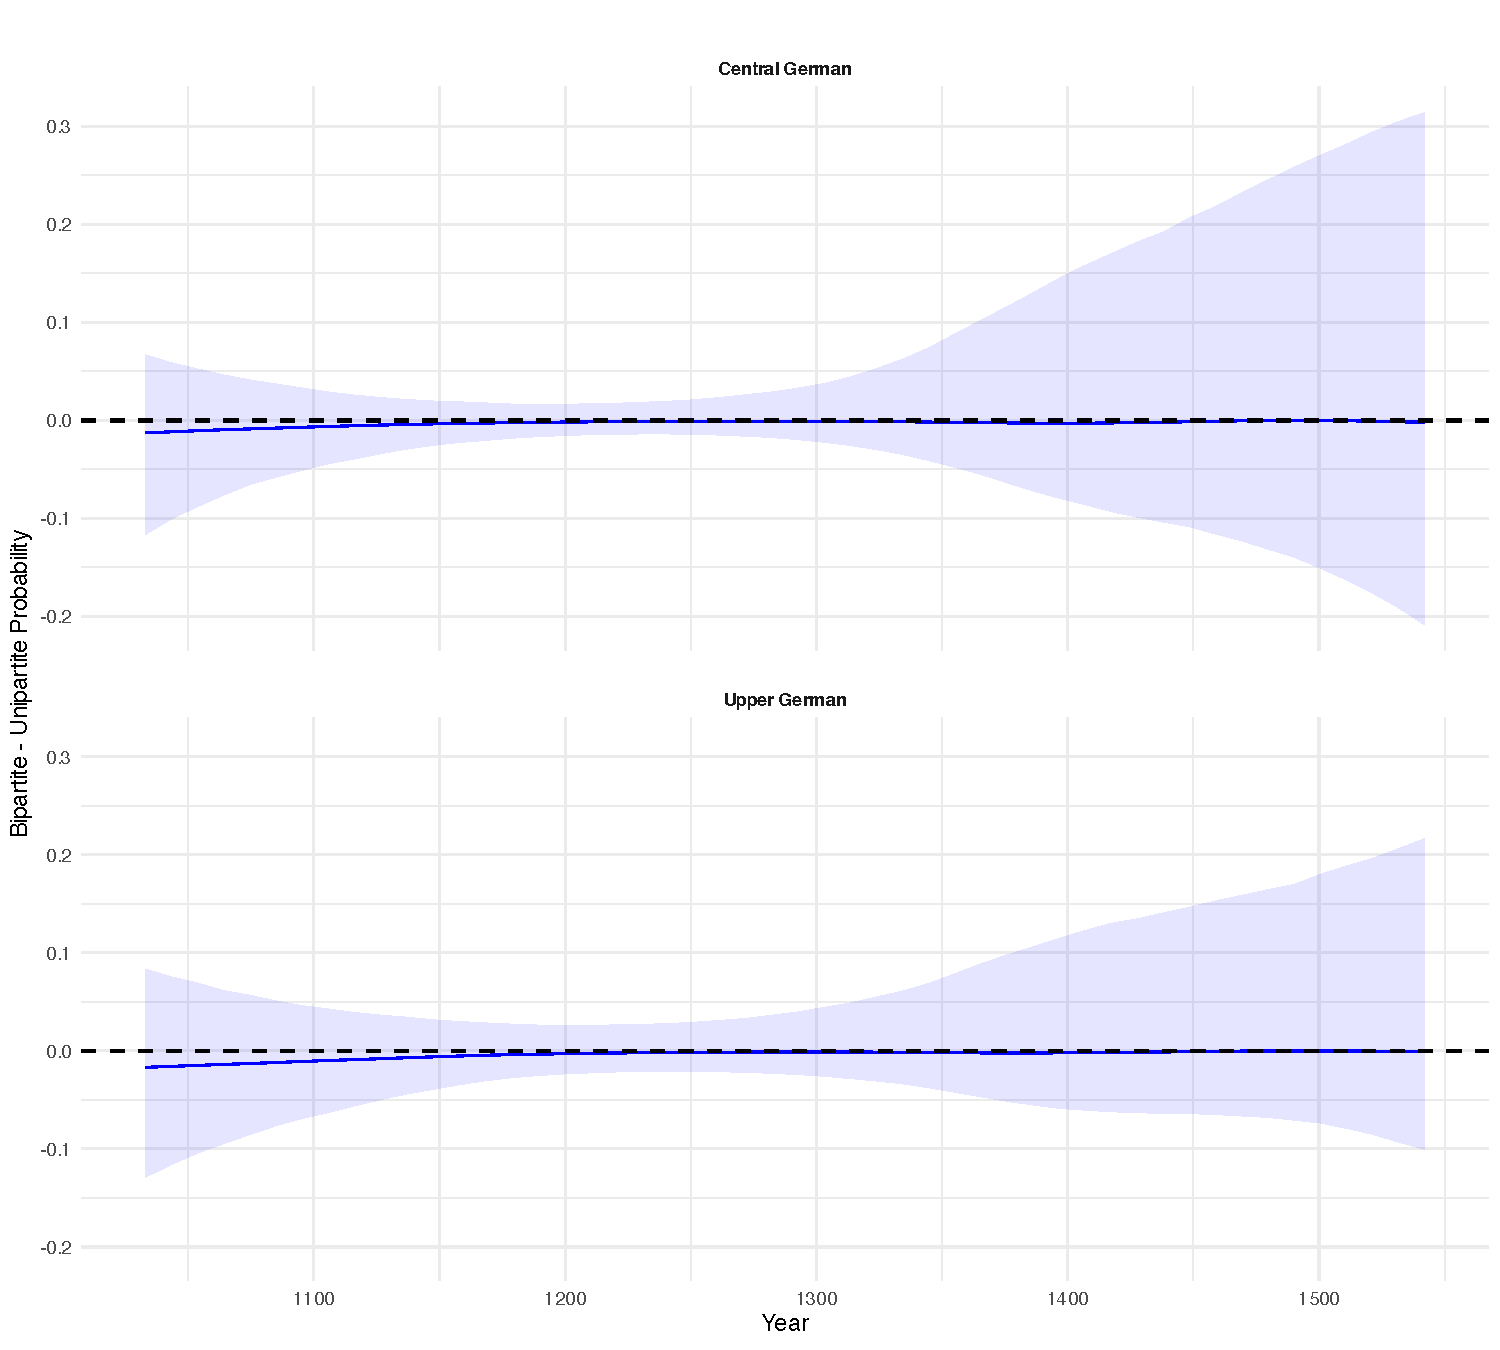
\includegraphics[width=0.7\linewidth]{figures/bi-uni_diff.pdf}
    \caption{Resistance to Leveling: Vowel Bipartite vs. Vowel Unipartite. Values lower than 0 represent support for Paul's Principle.}
    \label{fig:bi_uni_diff}
\end{figure}

When inspecting the dynamic of different marking types across time, we can confirm yet again the difference in levelling dynamics between vowels on the one hand and consonants on the other. The difference can be observed in Figure \ref{fig:level_trajectories}. The average probability of levelling for vowels does not change in a strong manner and only the uncertainty increases around 1400, while consonant levelling probability steadily increases after 1350 and 1500. 

\begin{figure}
    \centering
    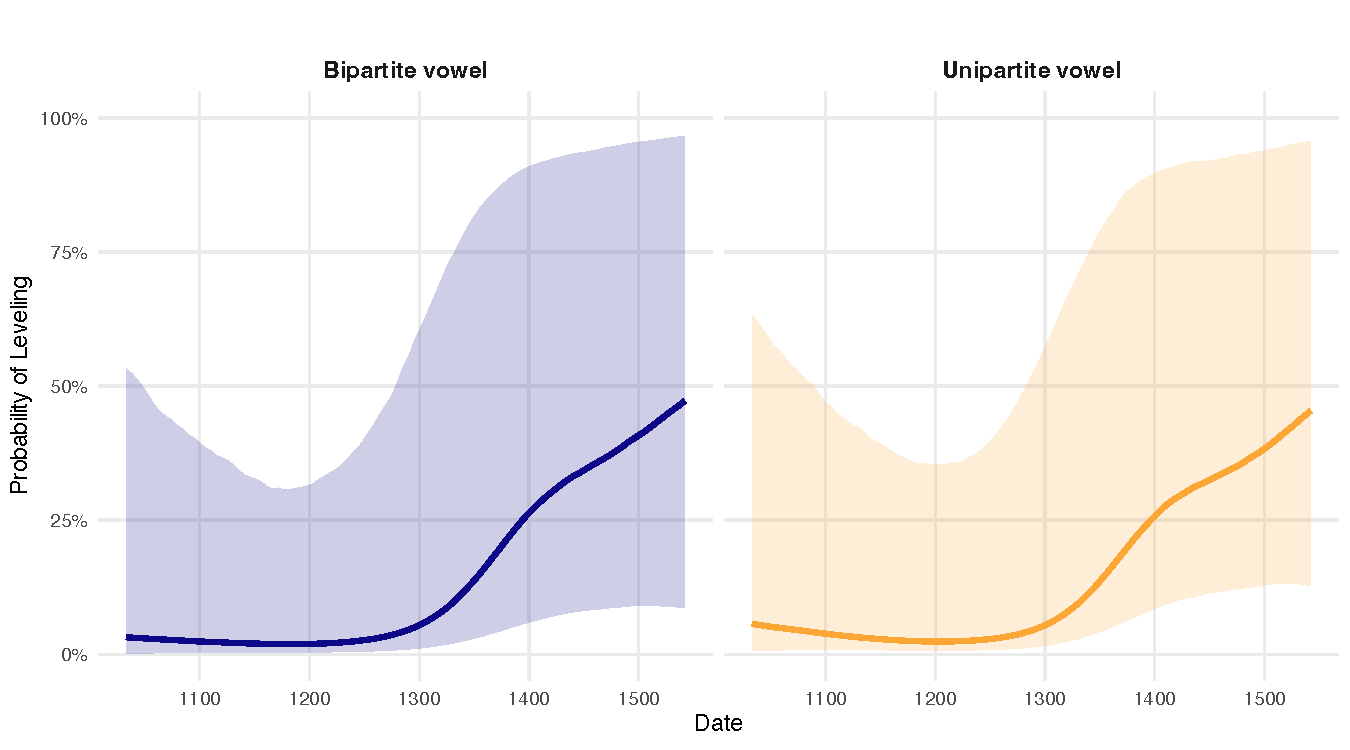
\includegraphics[width=0.85\linewidth]{figures/leveling_trajectories.pdf}
    \caption{Different marking type probabilities of levelling over time.}
    \label{fig:level_trajectories}
\end{figure}


The rest of the fixed effects also provide interesting insights into the factors behind the levelling in High German. They are illustrated in Figure \ref{fig:fixed_effects}. As has already been alluded to, the 95\% CI for both unipartite and bipartite vowels are strictly negative compared to baseline consonants highlighting again vowels' higher resistance to levelling. Interestingly, the only other variable to have a CI non-overlapping with 0 is the presence of alternation between the past singular and past plural subparadigms. The presence of alternation increases the probability of levelling which should be of no surprise, as modern day High German does not retain this alternation at all. According to our model and the data, it makes no difference whether the alternation pattern is frequent or not, it is simply its presence that increases the probability of paradigm levelling in the past subparadigm.

\begin{figure}
    \centering
    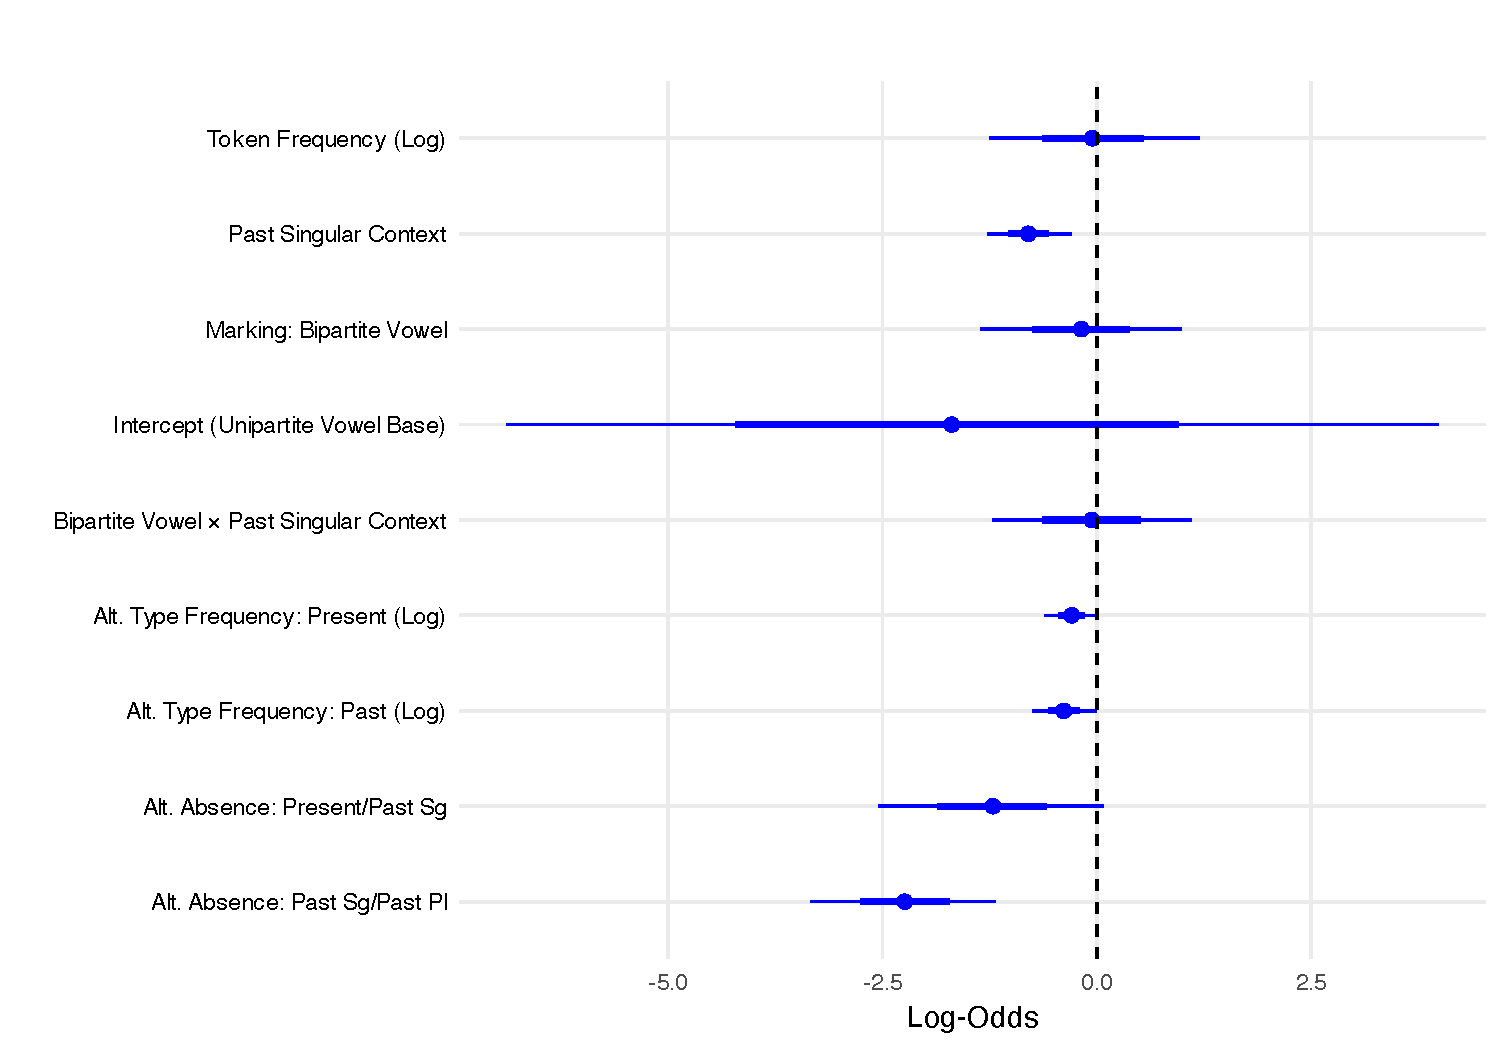
\includegraphics[width=0.85\linewidth]{figures/fixed_effects.pdf}
    \caption{95\% CI of posterior distributions for fixed effects.}
    \label{fig:fixed_effects}
\end{figure}

As can be seen from Figure \ref{fig:fixed_effects}, there is no effect of lemma frequency on the levelling probability. Marginal effects' 95\% CI includes zero and is centered around it $[-0.00155, 0.00406]$. The same is observed for token frequency $[-0.00712, 0.00256]$. However, there is an interesting difference that shows up when plotting the effect of lemma/token frequency across time as shown in Figure \ref{fig:freq_time}. The contour plots visualize the dynamic, two-dimensional interaction surfaces between temporal progression and frequency as captured by the tensor product smooths. The right panel demonstrates a classic conserving effect for token frequency: as morphological homogenization accelerates during the Early New High German period, items with lower token frequency (bottom right) become significantly more vulnerable to paradigm leveling than their high-frequency counterparts, which largely resist analogical restructuring. In stark contrast, lemma frequency (left panel) reveals a highly complex, non-monotonic relationship over time. Rather than acting as a universal conserving force, high lemma frequency paradoxically correlates with the highest probabilities of leveling toward the mid-16th century.

\begin{figure}
    \centering
    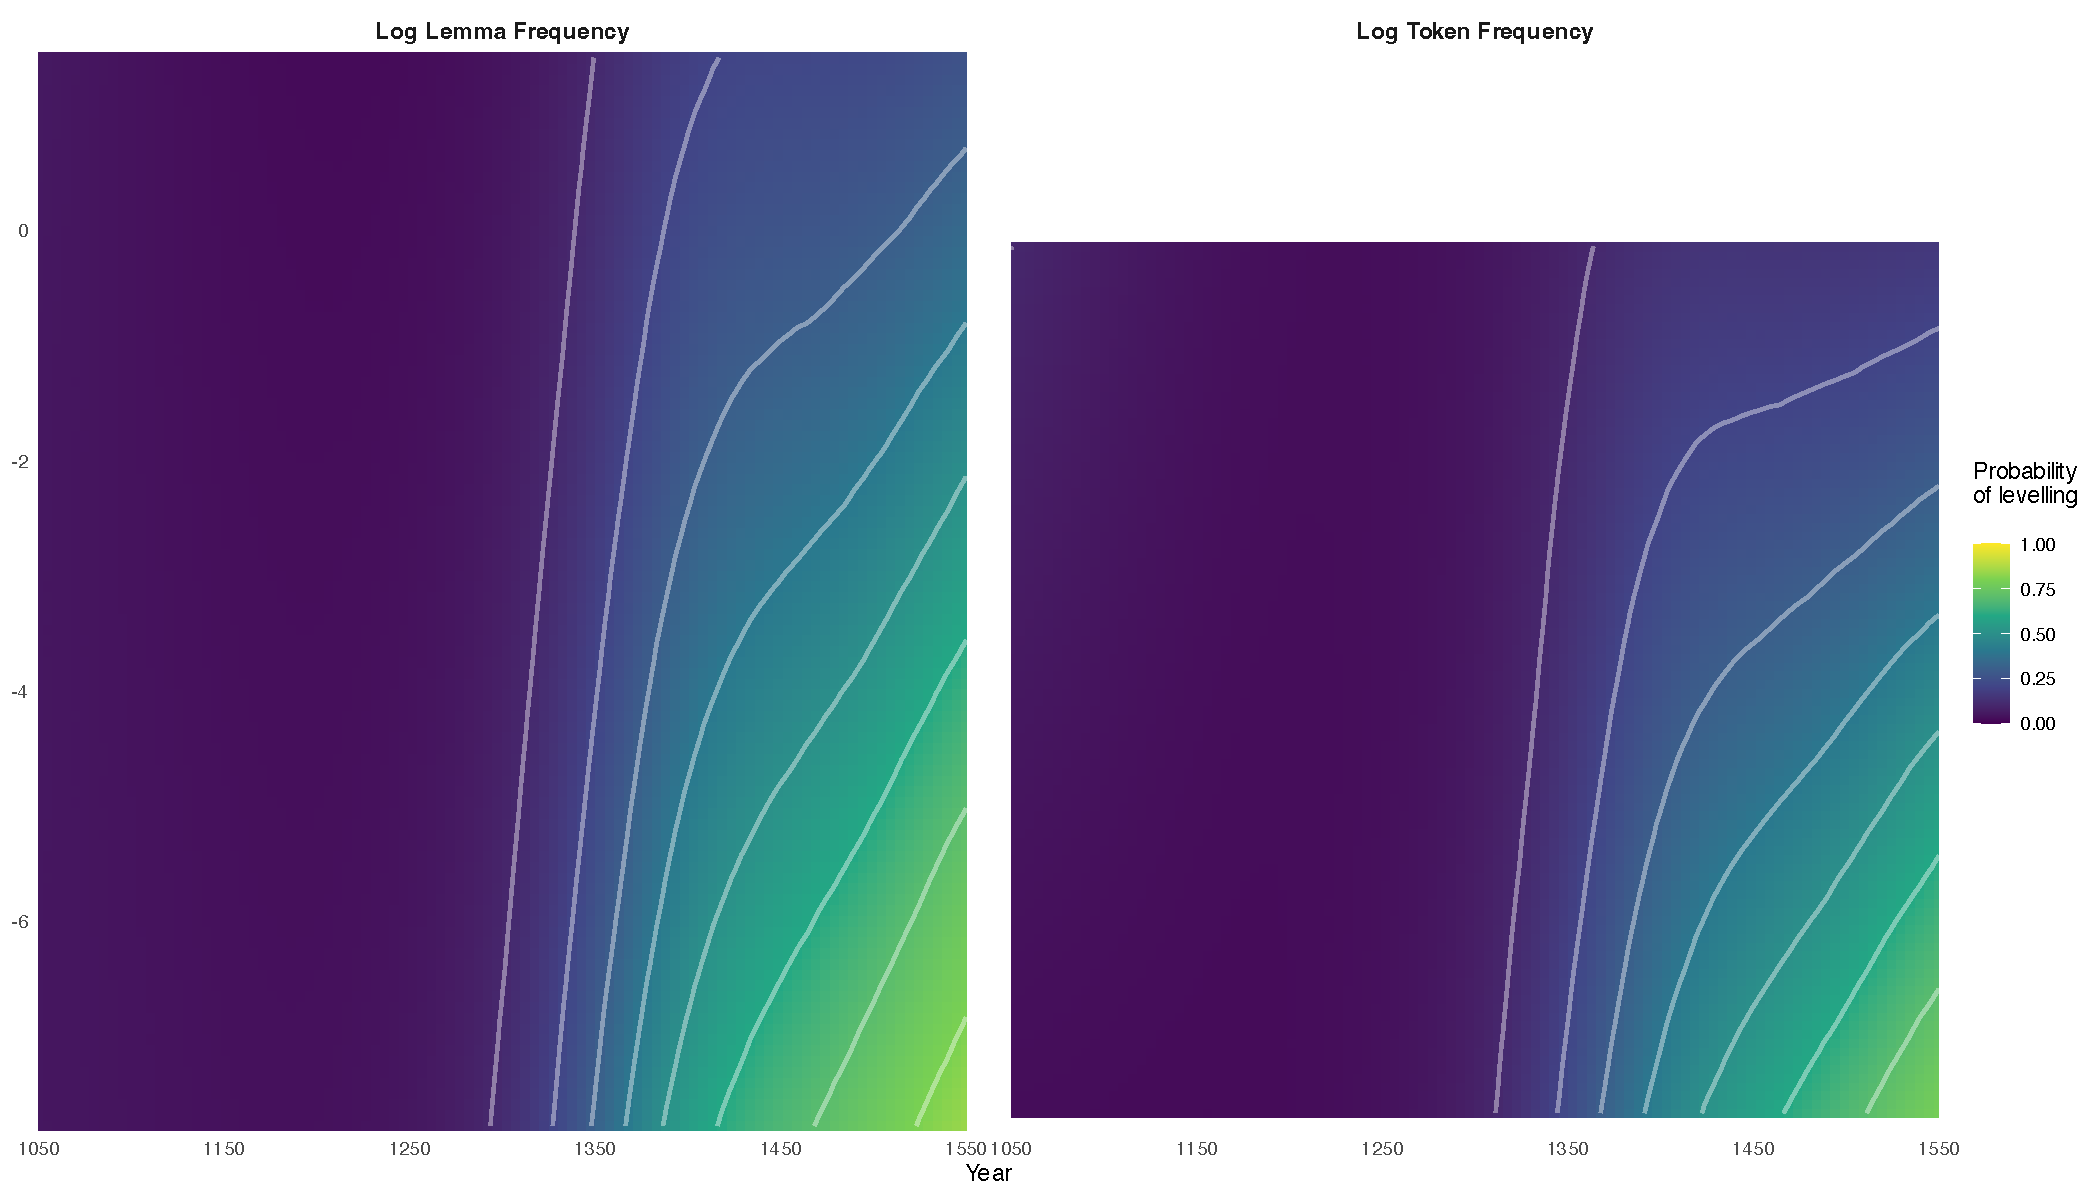
\includegraphics[width=0.85\linewidth]{figures/freq_time.pdf}
    \caption{Contour plots of the tensor product smooths demonstrating the interactive effects of time (Year) and log-transformed frequency on the probability of paradigm levelling. The color gradient and contour lines indicate the predicted probability. While token frequency (right panel) exhibits a consistent conserving effect against levelling in the late ENHG period, lemma frequency (left panel) displays a highly complex surface where high-frequency items ultimately show increased vulnerability to paradigm levelling.}
    \label{fig:freq_time}
\end{figure}


\section{Discussion}

The empirical results generated by our Bayesian Generalized Additive Mixed Models offer a compelling story about the historical dynamics governing paradigm leveling in High German strong verbs. Most notably, our findings provide no statistical support for Paul's Principle. The theoretical assumption that bipartite marking, defined as the co-occurrence of vocalic Ablaut and consonantal \textit{Grammatischer Wechsel}, establishes a heightened cognitive threshold of resistance against analogical leveling is not supported by our findings. The evidence ratio and the corresponding credible intervals indicate no meaningful difference in the leveling trajectories of vowels in bipartite versus unipartite paradigms. 

Rather than a broad, structurally determined resistance to leveling, the data reveals a stark asymmetry between the elements of the paradigm itself: vowels exhibit profound resistance to leveling, whereas consonants face aggressive morphological homogenization, particularly accelerating after 1350 CE. This element-specific vulnerability aligns neatly with modern psycholinguistic models of sequential speech perception and complex uniqueness points (CUP) \citep{cup_paper2008}. Because the root vowel precedes the coda consonant in the linear speech string, it provides an early, high-fidelity acoustic cue regarding the specific paradigm cell being accessed. Once the vowel resolves the informational ambiguity of the morphosyntactic category, the subsequent consonant alternation becomes informationally redundant. As discussed in \cite[pp.~102--121]{fertig2013analogy}, the leveling of alternations often coincides with the demise of their phonological motivation; once the \textit{Grammatischer Wechsel} became fully opaque and redundant to the heavily entrenched Ablaut, speakers systematically leveled the consonants to reduce unnecessary paradigmatic complexity. 

Perhaps the most surprising result of our model is the null effect of lemma frequency and token frequency on the probability of leveling. A vast body of historical linguistic and psycholinguistic literature posits that token frequency acts as a formidable conserving force, granting high-frequency items the "lexical strength" to resist analogical restructuring \citep{desmet_vandevelde2019, fertig2013analogy}. However, our analysis suggests that in the context of a systemic macro-shift, such as the total collapse of the singular/plural preterite split in ENHG, the global drive toward systemic congruity overwhelms the local protective effects of individual lemmas frequencies. This interpretation is supported by recent work on the Paradigm Cell Filling Problem (PCFP) \citep{annual_review_analogy2024}, which emphasizes that analogy is driven by the global predictability and implicative entropy of the inflectional system rather than the isolated lexical strength of specific lemmas. 

Notably though, we do find an effect of increased levelling probability if we inspect the results of the model that uses token frequency instead of lemma frequency. Lemma frequency aggregates the occurrences of all inflectional variants of a lexeme. While this is a useful metric for measuring the overall cognitive availability of a semantic concept, it obscures the realities of morphological processing.

As demonstrated by \cite{baayen_freq_2003}, stem (lemma) frequency is an excellent predictor for response latencies of base or singular forms, because the resting activation level of the access representation is a function of the summed frequencies of its inflectional variants. However, using lemma frequency to predict morphological change creates a statistical artifact. If a lexeme has a massive overall frequency, but the specific paradigm cell undergoing levelling (e.g., a 2nd person plural) is rarely used, a model using lemma frequency will treat the rare form as if it possesses the high frequency of its lemma. This aggregates highly entrenched forms with highly vulnerable forms, resulting in the noisy, distorted contours that can be observed on the left side of Figure \ref{fig:freq_time}.

Similarly, the specific type frequency of an alternation pattern was found to have no significant effect on its survival. Instead, it was the mere \textit{presence} of an alternation between the past singular and past plural subparadigms that significantly increased the log-odds of leveling. This targeted eradication of the number distinction within the past tense strongly supports the semantic homogeneity constraint, wherein speakers actively eliminate complex, arbitrarily nested allomorphy within a single, highly salient semantic domain (Tense) to restore a more transparent form-to-meaning mapping.

\subsection{Limitations and Methodological Considerations}

While the modeling architecture utilized in this study is robust, several methodological limitations must be addressed to properly contextualize the findings. The primary limitation stems from the inherent sparsity and uneven distribution of historical corpus data. To maintain sufficient statistical power, we abstracted dialectal variation into two macro-regions (Upper German and Central German). While this binary split successfully captures the broadest effects of the Second Consonant Shift and regional apocope/syncope, it inevitably glosses over micro-regional variations that could have provided localized phonological input for, or resistance to, analogical change.

A related constraint concerns the empirical basis of our central contrast. Bipartite paradigms are rare in the attested record: of the 88 lemmas that enter the model, only 11 are bipartite, and the \textit{vowel\_bipartite} category comprises 705 of the 13,184 observations, of which merely 3 are coded as leveled. Our test of Paul's Principle therefore rests on a sparsely populated cell. The weakly informative priors described above are centered on zero, and where the likelihood is this thin they pull the posterior toward the null. This shrinkage acts in the same direction as the conclusion we report, and we therefore state that conclusion in its appropriate form: the wide credible interval for the bipartite versus unipartite contrast reflects an absence of evidence for a protective effect, not positive evidence that the effect is exactly zero.
% OPTIONAL, to quantify the prior's contribution -- paste at the end of the paragraph above:
% The posterior standard deviation for this contrast is 0.94, against an implied prior standard deviation of approximately 1.41 for the difference of two \text{Normal}(0, 1) coefficients. The data thus constrain this particular comparison only partially.

Similarly, our operationalization of the morphological context into holistic "past singular" and "past plural" subparadigms is a necessary heuristic to combat sparse attestations of specific person-number cells. While this groups functionally equivalent historical stems, it assumes a uniform rate of analogical change across all persons within those numbers, potentially obscuring minor intraparadigmatic pivot effects.

Finally, as with any study utilizing historical corpora, we must acknowledge that written texts are fundamentally conservative proxies for the spoken vernacular \citep{desmet_vandevelde2019}. The S-curve of morphological leveling observed in our data (peaking around 1500 CE) likely lags behind the actual timeline of change in the spoken language. Nonetheless, the strict application of our sound-change exclusion dictionary ensures that the leveling tracked in our dataset represents genuine morphological reorganization rather than mere orthographic or phonological drift, providing a high degree of confidence in our rejection of Paul's Principle.
